\chapter{Conclusion: Paradigms and Possibilities}
%outline where the diss has been to set up some framing
The chapters of this dissertation build on one another to create what seems to be an isolated, self-supporting data pipeline in which terms like jazz, harmony, chord, progression, and function receive narrowly specific (and idiosyncratic) definitions.  Building a corpus of jazz performance in MIDI format, tallying tiny-duration, locally-transposed scale degree sets as chords, and clustering those chords based on the statistics of their temporal deployment produce jazz harmonic claims connecting analytical abstraction to performance data through a complex -- but transparent and consistent -- series of computational procedures.  It is clear that these claims are supportable within the sandbox given here; less clear is their status with regard to traditional theories of jazz (and non-jazz) harmony, since the preceding three chapters look quite different from traditional harmonic theory discourse.

What I advocate here, in its most generally Kuhnian sense, is a paradigm shift\footnote{Cite Kuhn, \emph{Structure of Scientific Revolutions}.}  Extant successful jazz harmonic theories employ a particular epistemic framework (or, more properly, a closely-related set of frameworks), a language in which to write claims, as I will discuss below.  At the ground level, these frameworks involve ways of defining the terms of the discourse, like ``chord" and ``progression," as well as the accepted data to which the claims of the discourse should be accountable, like ``lead sheets" or ``score transcriptions."  But any functional paradigm also consists of an agreed-upon set of production rules for claims, a series of methods or processes used to generate statements about the data in a discursively-stable way.  Put reductively, I consider a paradigm to consist of discursively-useful statements, a domain deemed relevant and appropriate for investigation, and methods which the community operating under the paradigm considers sufficient for furnishing a proof of or offering support for the discursive statements.

Theorists in any field may (and do) differ regarding which claims are ``true" under the paradigm, and this is the source of most productive academic discourse.  But when the claims written in a paradigmatic language become sufficiently complex, new paradigms may be proposed; as Kuhn notes, new paradigms typically gain supporters in the field by re-writing claims accepted under the old paradigm in terms of the new.  If the proponents of the new paradigm can demonstrate that the same (\emph{a priori} useful) claims are reachable in a new way, and if they can argue that the new paradigm provides a framework more flexible, generalizable, justifiable, or elegant, then segments of the discourse may migrate, choosing to identify problems, perform research, and present their results in terms of the new paradigm.  A paradigm shift may undermine few or none of the claims made in the old paradigm, replacing instead the assumptions underlying and language describing the claims.

Seen on this basis, three types of inquiry transpire in this dissertation:
\begin{enumerate}
	\item \textbf{Reproduced claims}: Much of the heavy-lifting of this dissertation results in reproducing old knowledge in new terms.  When chapters 3 and 4 produce clustered categories of phonetic and syntactic similarity, the results largely align with traditional expectations regarding tertian-stack, root-based, hand-analyzed category assignment.  Work of this kind reproduces statements like ``$I$ triads behave like $vi$ triads," but it does so by a completely different set of processes accountable to different data.
	\item \textbf{Unreproduced claims}: Some types of claim produced by other paradigms cannot be rewritten (either simply or at all) in terms of the framework established in the preceding chapters.  Some of these unreproduced claims demonstrate weaknesses in the new paradigm, places where it fails or requires supplementation.  Others might indicate failures of extant paradigms, claims which might fail to be reproduced because they are only consistent or relevant in the context of their particular frameworks.  Interpreting the status of unreproduced claims with regard to existing and new paradigms involves complex considerations of epistemology and discursive utility.
	\item \textbf{New claims}: The data-driven framework which allows the reproduction of many pre-existing claims also broadens the class of claims possible.  By stripping away assumptions about chord structure, root, and successive immediacy, constructing and examining temporal progression regimes affords statements ill-formed under other paradigms, including statistically-supportable claims about the behavior of chords at a distance and similarity measures between chords with arbitrarily different pitch structures.
\end{enumerate}
The first and third kinds of inquiry enumerated above represent a straight-forward argument for a paradigm shift in discourse on jazz harmony.  The second kind functions to destabilize the totalizing nature of that shift, pointing to the limits of the new paradigm and identifying places where other paradigms provide better, more nuanced, and more useful claims.  The examination of unreproduced claims encourages us to suspend judgment regarding which conceptual proof structures are valid in favor of imagining which kinds of discourse might accomplish worthy goals.

Chapters 2-4 largely constitute demonstrations of claim reproduction.  Chapter 2 extracts chords and voicings in line with the theoretical expectations of Mehegan, Martin, and Levine.  Chapter 3 translates notions of chord behavior into explicitly temporal syntactic terms, reproducing the most basic harmonic expectation found in elementary jazz harmonic discourse -- $ii - V - I$ -- from progression statistics in three temporal regimes.  With syntactic temporality as a ground, Chapter 4 reproduces chord categorization and substitution schemes employed by theorists like Strunk and Levine.  If these kinds of claims have discursive utility, attending to temporal progression regimes clearly affords their reproduction, albeit from a different domain -- a highly individualized corpus of unquantized MIDI performance, rather than notational transcriptions of tunes or recordings -- and with a different idea of what furnishes proof -- statistics produced without hand-annotation.

In what follows, I will compare my work to the work of other jazz theorists, paying particular attention to existing claims unreproduced under my temporal syntactic paradigm.  I will then suggest new types of claim that paradigm allows, noting the productive potential afforded by supplementing the shortcomings of explicit temporal syntactic statistics with complementary analytical frameworks.  At the end of the chapter, I will suggest (somewhat paradoxically) that the very nature of a data-driven, corpus-based paradigm might amplify the impact of destabilizing, unreproduced claims, rendering the heterogeneous remainders left behind by dominant paradigms more legible and accessible.  Data-driven harmonic analysis might be seen to provide tools capable of both making powerful generalizations and undermining their hegemonic influence.

\section{Unreproduced Claims: Comparing frameworks}
%But how do we pull apart the structure of the old paradigm, theoretically?  Close reading of Strunk, Waters, and Terefenko.
%Pull in Wollheim's types of formalism

While claims regarding the typical deployment of chords with respect to their local key centers are well-captured by na\"{i}ve temporal clustering, several related types of harmonic claim find no ready translation.  Two traditional discursive methods -- that of discussing harmonic prolongations, and that of performing close score analysis of functional harmony -- do not exhaust the space of unreproduced claims, but they may capture the most important omissions.  Understanding the nature and interpretation of unreproduced claims from these frameworks requires an examination of more than the intuitive usefulness of the claims themselves.

Both theoretical processes partake of what might be called \emph{formalism} in particular ways, abstracting harmonic claims from the musical surface meant to capture information about performance independent of a variety of other contextual factors and features.  These abstractions, reductions, and partitions of features are not entirely unique to the musical domain, and in discussing them, I will make reference to the descriptions of analogous formalism in the theory and history of art offered by Richard Wollheim.\footnote{Cite Wollheim, especially \emph{Formalism and Its Types}, and to a lesser extent \emph{Art and Its Objects}.}  Following the mid-century backlash of syntactic and symbolic formalists against early twentieth-century biographical intentionalism,\footnote{By this, I mean the wave of formalist projects in the 1950s and 1960s which share George Kubler's eloquent description of art praxis as a dark mine; for Kubler, investigating the personal histories of the individual artists-\emph{cum}-miners precludes an appropriate focus on the (formalist) nature of the composition and topography of the material available for mining.  Kubler's work presents a complex historical formalism, and his abstraction of stylistic change in terms of mathematically-inspired chains of replication is ultimately brought into contact with Wollheim's formalist critiques in the work of Whitney Davis.  See Kubler, \emph{The Shape of Time}, and Davis, \emph{Queer Beauty} and especially \emph{A General Theory of Visual Culture}.}  Wollheim offers a series of corrective critiques regarding the formalist (over)reaction.  Concerned with art-historical claims regarding the ``essence" of particular works of art as being fully separable from and analyzable without representational or historical information, Wollheim offers in \emph{Formalism and Its Types} an analytic typology of formalisms, each type of which warrants specific structural objections.

In what follows, I will bring Wollheim's notion of manifest formalism to bear on the jazz prolongational work of Steven Strunk and its response and elaboration in the work of Keith Waters.  Waters's nuanced position will lead to a discussion of latent formalism in jazz harmonic analysis, and I will follow Wollheim's description of particularly syntactic latent formalism to situate my harmonic claims with regard to close readings and pedagogical techniques offered by Darius Terefenko.

\subsection{Prolongation as Manifest Formalism}
%Strunk jazz prolongation, Waters's response, translation into Wollheim
%manifest formalism as drive-by attack on Schenker, pivot toward latent formalism

%Strunk
The Spring 2016 issue of \emph{Music Theory Spectrum} offers an unusual chance to compare very similar jazz harmonic analyses from two different scholars which differ primarily in their justification schemes.  Published adjacent to one another, Steve Strunk's ``Tonal and Transformational Approaches to Chick Corea's Compositions of the 1960s" and Keith Waters's response, ``Chick Corea and Postbop Harmony," both engage with the harmonic language of Corea's ``Windows" (1966).\footnote{Cite Strunk and Waters.}  The published lead sheet for the tune is reproduced here as Figure~\ref{windows}.  In an attempt to explain the ``tonal and harmonic ambiguity" of ``Windows," Strunk provides Schenkerian voice-leading graphs and layered harmonic reductions based on Corea's published lead sheet for the tune.  The two analytical possibilities Strunk offers for ``Windows" both foreground substantial prolongations of E Major (which Strunk labels as a global $IV$); his ``middleground graph 1", reproduced in Figure~\ref{strunk_fig}, prolongs E Major from m.\ 17 all the way through m.\ 45-- more than half the tune's length-- while the alternate ``middleground graph 2" ends the prolongation at m.\ 33.  In both cases, this prolongation provides a ground for Strunk's claim that the 8 measure long alternation between $A\flat^7$ and $A^7$ consists of a nonfunctional embellishing chord ($A\flat^7$) which itself receives an embellishing chromatic upper neighbor ($A^7$, which Strunk suggests may also ``be thought of as a substitute dominant replacing $E\flat^7$, $V$ of $A\flat$").  Strunk's graphs present a clear hierarchy of tonal regimes, where $Bm$ (or $BM$, later) and $EM$ provide the context necessary for parsing the surface-level harmonies of the tune.

%Windows lead sheet
\begin{figure}
	\centering
	\caption{Strunk's Figure 1, the published lead sheet for Chick Corea's ``Windows."  Taken from p.\ 17 of Strunk (2016).}
	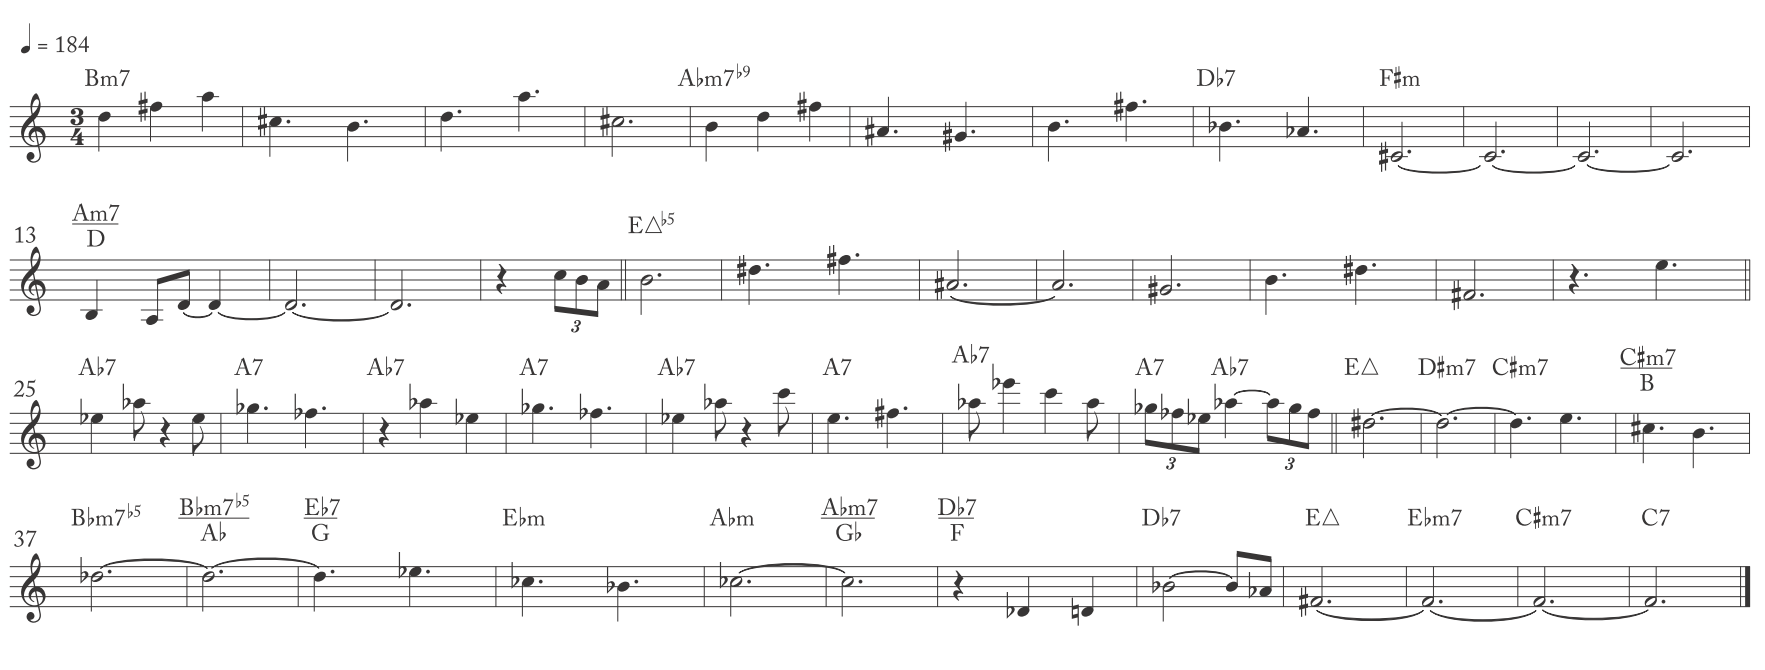
\includegraphics[width=6.4in]{strunk_windows.png}
	\label{windows}
\end{figure}

%Strunk's middleground 1 with extended E prolongation
\begin{figure}
	\centering
	\caption{Strunk's Figure 2, his ``Middleground graph 1" for Corea's ``Windows."  Taken from p.\ 18 of Strunk (2016).}
	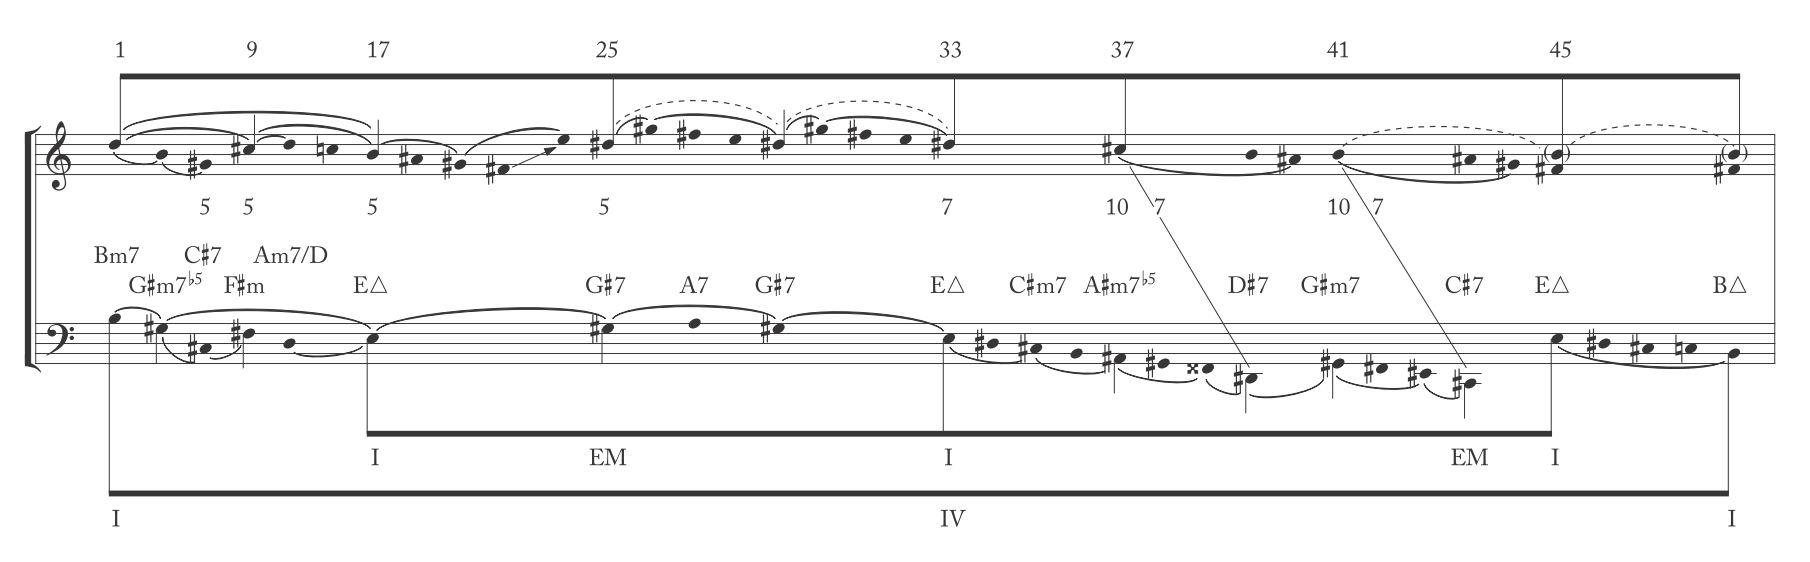
\includegraphics[width=6.4in]{strunk_windows1.png}
	\label{strunk_fig}
\end{figure}

%Waters
Waters re\"{e}xamines ``Windows" with skepticism regarding the importance of $IV$ as a functioning tonal subdominant, opting instead to describe the piece as a series of ascending fifth-related keys poorly captured by an appeal to the subdominant (or indeed by a monotonal reading in general).  Parsing the tune through the lens of a repeated ascending-fifth ``schema" drawn from Bill Evans's ``34 Skidoo," Waters rehabilitates many of Strunk's embellishing chords as essential stepping stones for a schematic sequence -- $Bm$, $F\sharp m$, $C\sharp m$, $A\flat m$ -- encompassing measures 1-41.  Waters labels the successive ascending-fifth phases of the tune in his Example 2, reproduced here as Figure~\ref{waters_fig}.  Tracing the fifths through the entire tune requires the abandonment, or at least the substantial weakening, of Strunk's $EM$ tonal prolongation.

%Waters's four-stage ascending-fifth schema parsing of Windows
\begin{figure}
	\centering
	\caption{Waters's Example 2, where he parses ``Windows" as a series of ascending-fifth motions.  Taken from p.\ 40 of Waters (2016).}
	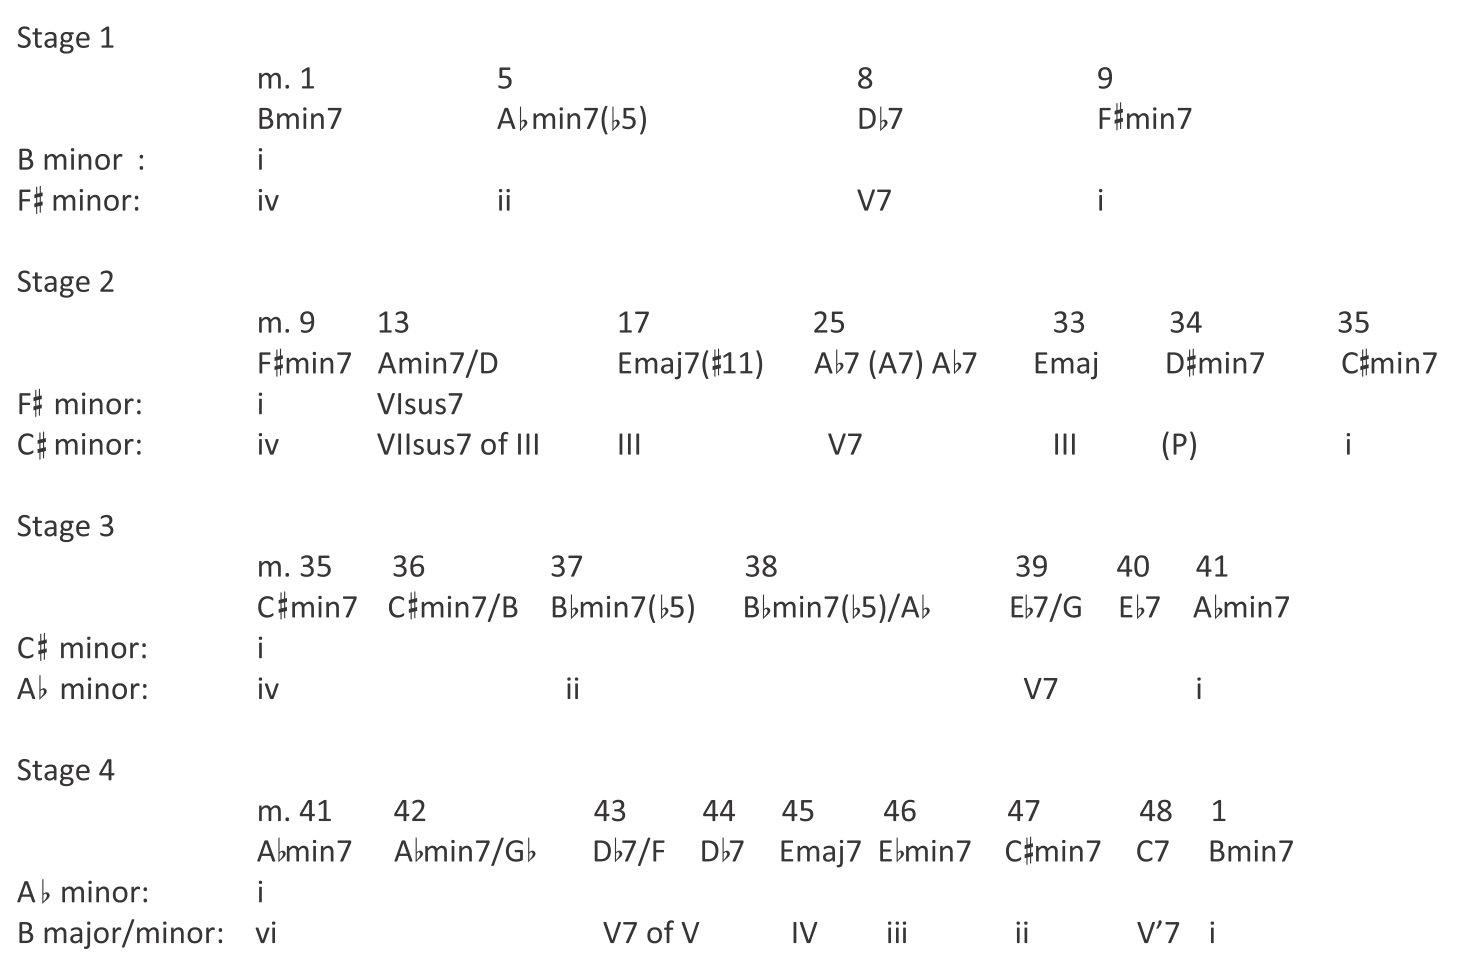
\includegraphics[width=6.4in]{waters_windows.png}
	\label{waters_fig}
\end{figure}

Waters notes that there are certainly ``compelling reasons" for Strunk's focus on $EM$, including its obvious duration, its hypermetrical placement at the start of two 8-measure phrases, and its appearance at both the beginning and ending of the hypothesized prolongational span.  But here, Waters objects on formal grounds, noting that ``neither duration, hypermetric inflection, nor departure/return is sufficient for prolongation."\footnote{Waters, p.\ 40.}  The usual grounds for prolongation -- presumably, embellishment through common passing or neighbor chords -- are missing, since the prolongation ``is carried out in an unorthodox manner, through $A\flat^7$ (mm.\ 25-32), a harmony in chromatic third relationship with E."\footnote{Waters, p.\ 40.}  Instead, Waters proposes that we hear $EM$ as a relative major substitute for $C\sharp m$, casting his re-labeling as a claim of harmonic relation and temporal delay: ``Thus the mm.\ 33-35 progression EMaj7 - D$\sharp$min7 - C$\sharp$min7 stands for C$\sharp$ minor (with ``stand for" meaning a transformation that meaningfully relates to and delays the more expected C$\sharp$ minor)."\footnote{Waters, p.\ 41.}  If the $EM$ sonorities have a ``function" in the tune, its primary status is not that of the subdominant of $B$, but rather as a substitute local tonic in $C\sharp m$.

%Waters:Strunk::Wollheim:Loran
I find Waters's analysis rewarding and attentive to the schematic norms of postbop practice, and I will return to his notion of substitutability and ``standing-for" in the next section.  For now, it suffices to note that his specific objections to Strunk's analysis echo Wollheim's description and critique of manifest formalism in the work of art critic Erle Loran.\footnote{The Loran discussion comes in \S 12, pp.\ 22-26, of \emph{On Formalism and Its Kinds}.}  In summarizing the argument of Loran's 1943 book on C\'{e}zanne's practice, Wollheim describes a reduction and justification process similar to Strunk's Schenkerian parsing: beginning with C\'{e}zanne's \emph{Still Life with Faience Jug}, reproduced here as Figure~\ref{cezanne}, Loran provides a reductive analytic overlay, isolating and extracting what he sees to be the formal boundaries or outlines of shapes given in the painting.  He then draws ``carry-through" lines designed to track and describe representational, volumetric tension experienced by a viewer.  The two-dimensional outlines give rise to (or represent) some phenomenal three-dimensional volumes, and those volumes are relatable to one another in a formal way.  All of this, Loran states, can be gleaned from the purely configurational (that is, formal, content-free) aspects of the painting.  Wollheim reproduces several of Loran's supporting diagrams, four of which appear in Figure~\ref{loran_diagrams}.

%the cezanne painting
\begin{figure}
	\centering
	\caption{C\'{e}zanne's \emph{Still Life with Faience Jug and Fruit}, from the Oskar Reinhart Collection ``Am R\"{o}merholz," Winterthur.}
	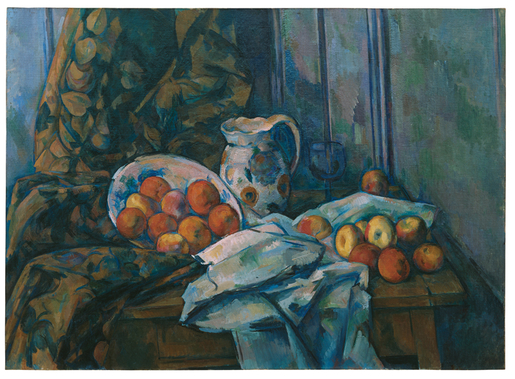
\includegraphics[width=6.4in]{cezanne.png}
	\label{cezanne}
\end{figure}

%the Loran diagrams
\begin{figure}
	\centering
	\caption{Four of Erle Loran's C\'{e}zanne diagrams, taken from Wollheim (1995), pp.\ 44-45.}
	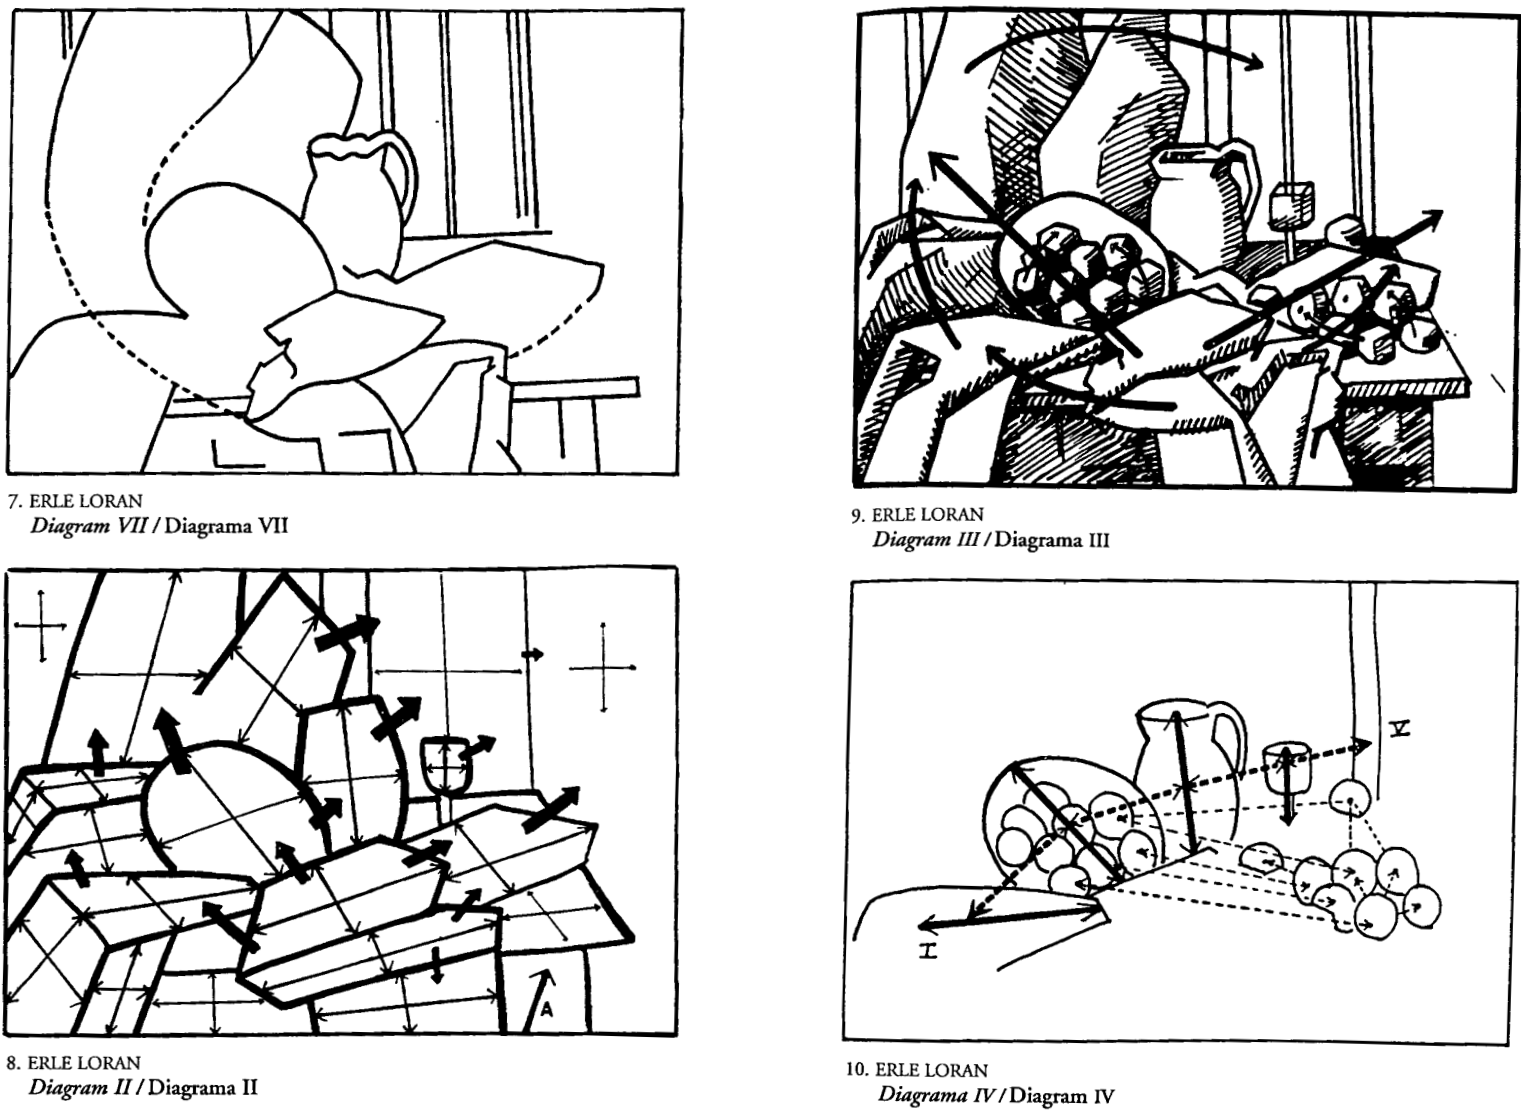
\includegraphics[width=6.4in]{loran_diagrams.png}
	\label{loran_diagrams}
\end{figure}

Wollheim has two main objections.  First, and more generally, he doubts that the outlines of shapes can be reliably extracted from a painting in a consistent and purely formal way, without explicit appeal to the representational content of some viewer.  Judging where a shape begins and ends, Wollheim reminds us, is strongly informed by our internalized norms for the properties of whatever shape(s) and represented object(s) we might recognize in a given visual array.\footnote{Consider Wollheim's discussion of identifying the ``black ring" crowd shape in Breughel's \emph{Christ Carrying the Cross to Calvary} on pp.\ 9-13.}  Second, Wollheim drives a wedge between the two-dimensional outlines and Loran's ``carry-through" lines of three-dimensional tension.  Loran claims that the volumes arise from the formal configurations of the two-dimensional shapes, but Wollheim counters that the moment of turning a two-dimensional array into a represented three-dimensional volume is a psychological one, and that it cannot possibly occur independently of the other (non-formal) aspects of the painting.  As Wollheim puts it in his general rebuttal to manifest formalism, of which he sees Loran's work as a particularly problematic variety,
\begin{quote}
``Observe the earthenware object that lies on the ground on the left-hand side of the picture [Breughel's \emph{Christ Carrying the Cross to Calvary}].  As our eyes alight on it, we recognize it as a domestic vessel.  At this point the beliefs that we have about such utensils confirm us in seeing the dark circle on its body as an aperture opening inwards rather than as a protuberance pushing outwards... [W]e cannot exclude from the formal aspects of the painting any factor that influences what we see in the painting.  And there seems no way in which we can be certain, in advance of particular cases, particular paintings, that some given aspect of a painting will never be such a factor."\footnote{Wollheim, \emph{On Formalism and its Kinds}, p.\ 22.}
\end{quote}
If Loran's three-dimensional tension is meant to arise from ``the similarity in the objects' size, shape, and colour," Wollheim suggests, ``we know better."\footnote{Wollheim, \emph{On Formalism and its Kinds}, p.\ 25.}  Noting visual tension between apples in two different locations in C\'{e}zanne's \emph{Still Life with Faience Jug} seems to involve more than familiarity with outlines and colors.  The identification of representational volumes based on shapes in the visual array, the tensions between those volumes, and even the boundaries of two-dimensional shapes themselves depend on more than just the formal features of the painting \emph{qua} painting: the viewer's multifaceted visual processing both requires and imposes numerous potentially non-formal aspects for and on any particular ``formal" parsing.\footnote{Wollheim's ultimately psychoanalytic commitment to the process of seeing-in and seeing-as is quite complex, and he would likely resist my use of the term ``parsing," here.  His formalist critiques do not necessarily depend on the adoption of his strikingly Freudian psychoanalytic representational stance, a thorough consideration of which may be found in Whitney Davis's \emph{Queer Beauty} (2010), chapter 10.}

With the caveat that translation of Wollheim's argument into musical form requires both nuance and skepticism, Waters's response to Strunk can be paraphrased in Wollheim's terms and leveraged toward a paradigmatic critique.  Like Wollheim's manifest formalists, Strunk purports to examine the musical surface and extract (trace) the important harmonies, those that control, prolong, or function as boundaries for tonal spans (shapes).  Reducing away voicings and embellishing chords, Strunk shows an E Major ``shape" as an important formal property of Corea's tune.  With attention to schema drawn from jazz practice, Waters sees a different tonal shape in the passage, and he challenges Strunk's identification of an EM prolongation in a way directly analogous to Wollheim's critique of Loran: Strunk's identification of the formal prolongation seems based on important musical aspects which are, nevertheless, not ``sufficient for prolongation."  To see the shape of the tonal prolongation Strunk identifies, we cannot simply extract surface-level chords to provide a formal justification; like with C\'{e}zanne's apples or Breughel's jug, our identification of the prolongation is dependent on features other than surface harmonic analysis.  If those other features are the ground on which the prolongation rests, no diagram of the type Strunk offers can furnish sufficient proof of its existence.  To put it in Wollheim's words:
\begin{quote}
``Though, through the use of diagrams, [Loran] can analyze, on the one hand, how the artist organizes the picture-plane and, on the other hand, how he organizes the represented space, what, in the nature of things, Loran cannot present diagrammatically is the meeting-point of the two, which is, for him, precisely where C\'{e}zanne's pictorial achievement, indeed pictorial achievement in general, lies... In order to grasp just how C\'{e}zanne fused the organization of volumes and the organization of the picture-plane, we have to go back to the painting itself and experience the fusion: nothing else will do.  There is no formulaic representation of the crucial stage."\footnote{\emph{On Formalism and Its Kinds}, pp.\ 24-25.}
\end{quote}
Since Strunk's prolongational reductions do not represent the moment where the surface harmonies somehow generate or map onto the tonal prolongation he suggests, the prolongation itself can be challenged.  Waters can provide an explanation appealing to a totally different paradigm: the passage might not need to form the shape of a tonal span in the subdominant, but rather could be seen as a series of ascending fifths.

%paradigm comparision, Schenkerian drive-by
The paradigms in play, here, make use of different terms and proof structures-- they start from different ``shapes," and they ``trace" those shapes in different ways.  Strunk's Schenkerian reductions begin with harmonic norms drawn from tonal, western-classical music, and they demonstrate a kind of tonal coherence by selecting surface features from ``Windows" to generate a hierarchy of important tonal features and regions.  Waters's schematic analyses begin with harmonic schema drawn from postbop jazz, and they demonstrate a replicatory chain of influence by interpreting surface voicings in a way designed to show their compatibility with repeated application of the same schema.

The statistical analyses of the preceding chapters cannot reproduce manifest formalist claims of the variety employed by Strunk and other Schenkerian-prolongational theorists.  And while these un-reproduced claims count against a temporal-syntactic paradigm, in one sense, they may be unreproducible for good reason: it may not be possible for data drawn from the surface-level harmonic content of jazz performances to demonstrate Schenkerian claims of tonal harmonic prolongation.  Waters's claims, to the extent that some of them are predicated on parsing jazz progressions in terms of repeated harmonic schema, may lend themselves to a corpus-syntactic paradigm more easily; as such, they (and my own claims) may resemble what Wollheim calls \emph{latent} formalism.

%More on latent formalism/positioning Waters here, or later?
%Might be good to have KW come back after Terefenko, in the heat of latent formalism

\subsection{Functional Analysis as Latent Formalism}
%Finish up Waters as grammatical/quasi-statistical latent formalist
%Terefenko's functions as syntactic latent formalism
%Wollheim's segmentation objection as motivating my project, which doesn't completely solve the problem

%Start with Terefenko-style functional analysis claims
If Strunk's prolongational analysis of Chick Corea's ``Windows" can be described as a kind of manifest formalism, as my Wollheimian extension of Waters's response implies above, it stands as one type of claim regarding jazz harmony unreproducible under the corpus-syntactic paradigm of chapters 2-4.  Manifest formalism does not exhaust the space of unreachable claims, however; two other paradigmatic modes of discourse on jazz harmony seem not to find a statistical home -- pedagogical approaches and functional analyses of individual tunes or performances.  As an exemplar for both of these varieties of inquiry, I turn below to Dariusz Terefenko's \emph{Jazz Theory: From Basic to Advanced Study} (2014).  I aim to unpack Terefenko's textbook partly as a latent formalist project, in Wollheim's terms, and I will ultimately suggest that my own work inclines in this direction, as well.

Terefenko does not aim his book at music theorists, at least not directly; rather, the text is meant for dedicated, adventurous musicians, ``undergraduate and graduate jazz students, and for an ever-increasing population of classical students interested in jazz theory and improvisation."\footnote{Terefenko, p.\ xv.}  As such, the book takes a fair amount of western-classical theoretical assumptions as a ground, providing quick primers on scales, meters, triads, and roman numeral analysis designed as reminders rather than explicit theoretical claims.  Since Terefenko presents theory in the service of practice, I will not subject his claims to quite the same critical attention as those in theoretical works like Strunk's or Waters's.  But attending to the model implicit in most of the book will, nevertheless, clarify one of the major presentational paradigms in jazz pedagogical literature.\footnote{For other, similarly latent-formalist and pedagogical examples, see ?????}

While Terefenko's descriptions for phrase models and song forms presented in Part Three invoke Schenkerian techniques, the earlier portions of the book treat prolongation with a light touch, instead presenting a wide array of chords through the lens of functional categories.  Terefenko describes harmonic function quasi-grammatically from the outset:  after introducing tonic, predominant, and dominant as the necessary components (or ``contextual features") of functional tonality, he describes their interrelated tension and release patterns in traditionally energeticist ways.  The restful stability of the tonic, the moving-away of the predominant, and the tense instability of the dominant are all ``different behavioral patterns," which ``remain constant across the entirety of the tonal system in which jazz forms a distinctive musical language with its own harmonic grammar and melodic syntax."\footnote{Terefenko, p. 26.}  But even as Terefenko firmly grounds jazz harmonic function within a western-classical tonal paradigm, he makes space for its own idiomatic dialect: ``As will be demonstrated time and time again, functional tonality in jazz has different properties than that of common-practice classical music.  These properties are represented by a unique set of rules dictating the unfolding of harmonic function, voice-leading conventions, and the overall behavior of chord tones and chordal extensions."\footnote{Terefenko, p.\ 26.}  Much of the rest of the book is dedicated to stipulating these rules and showing examples of jazz harmony's idiomatic grammaticality.

%Use Wollheim to describe them as latent formalism
As Terefenko assigns a plethora of jazz chords to the three basic functional categories, he builds the lexicon of a complex grammatical system with a comparatively simple syntax.  The tonic, predominant, and dominant, which exist as idealized parts of musical speech, occur in a small number of grammatical orderings; most of the interest in jazz harmony, for Terefenko, consists of complicated mappings from increasingly dissonant chords to their interpretive functional categories.  Parsing musical surfaces toward this end produces what Wollheim would call a latent formalist system, where the harmonic drama arises from the underlying syntax of progressions.  Wollheim offers an extremely clear description of linguistically-inspired latent formalist models, claiming that rules of syntactic organization must meet five requirements:
\begin{quote}
(one) they presuppose some way in which larger units can be segmented into smaller units, and ultimately into basic units;

(two) they then operate on the basic units, which they first classify under certain general categories.  In the case of language, examples of such categories are noun, verb, adverb;

(three) they order these elements, classified by category, into strings of elements that are well-formed, or grammatical, while all other strings are ill-formed, or ungrammatical;

(four) the rules function recursively, in that they can be endlessly reapplied to their own output so as to yield an unbounded set of further well-formed strings; and

(five) in those cases where the strings refer, or have a semantic dimension -- that is, in all cases except purely formal languages -- the meaning that each string has is determined by its syntactical form plus the vocabulary, or lexicon, of the language.\footnote{Wollheim, pp. 26-27.}
\end{quote}
Terefenko's functional harmonic syntax engages with each of these requirements.  He explicitly states that passages of varying length can carry functions or be divided into elements which do so; he classifies those harmonic elements into functional categories; he deploys the elements (usually chords) in well-formed progressions, repeatedly and with variation.  If Terefenko's musical strings (usually harmonic progressions) do indeed refer, along the lines of Wollheim's fifth requirement, their semantic dimension might encompass a particular tune or style of playing, both of which are presumably recognizable from the combination of functional syntax and a particular lexicon, be it voicings or head changes.  But setting aside musical semantics, a proper analysis will reveal the hidden (latent) syntax of a given passage, and a proper composition will follow the grammatical production rules for ordering categories to produce an intelligible tune or improvisation.

For formalist projects of this general type, Wollheim offers another critique.  Taking to task Yve-Alain Bois's semiological description of Picasso's Cubism, Wollheim shows that a supposedly-syntactic analysis of Picasso's \emph{Head of a Girl} or Grebo mask must fail to satisfy the requirements given above.  Three of Wollheim's objections find possible counter-arguments in Terefenko's syntax.  Wollheim claims that Bois ``proposes no categories analogous to those of grammar," while Terefenko does; Bois offers no rules for how to concatenate categories, while functional harmony does this, in a general sense; and Bois offers no sense of what un-grammatical works of art might be: ``He gives us no reason to think that pictorial objects can be divided into the well-formed, which are legitimate, and the ill-formed, which are illegitimate, where this division is effected on the basis of whether or not rules of a very specific kind have been properly applied in their production."\footnote{Wollheim, p.\ 30.}  If one of Terefenko's students is expected to improvise with other musicians and write tunes in a mutually-understandable idiom, there may well be social and grammatical norms separating well- and ill-formed utterances.  Functional harmonic latent formalism, it seems, avoids many of Wollheim's objections.

Terefenko's functional syntax may not, however, satisfy one of Wollheim's objections:  Wollheim complains that Bois offers ``no systematic way in which the total surface of the pictorial object could be segmented-- segmented, that is, without remainder-- into parts, which could then function as syntactical constituents."\footnote{Wollheim, p.\ 29.}  When confronted with a complex visual array, a Boisian latent formalist must somehow decide how to chop up the painting into syntactic elements and how to recognize each element as part of the appropriate grammatical category.  This segmentation difficulty has an auspicious musical history in atonal music theory,\footnote{See some citations of the segmentation problem inherent in pc-set theory.} but it applies to Terefenko's contextual parsings, too.

As one parsing example among many, consider Terefenko's statements regarding how to parse the simple tonal progression on his p.\ 33, reproduced here as Figure~\ref{Terefenko_ex}.  Several of the chords can be given \emph{a priori} functional assignments based on their pitch structure -- in the limiting case, Terefenko has given the student no category other than tonic for the minor $i$ chord, but $V$ and $ii^\circ$ also seem unambiguous, here.  The $VI$ chords of measures two and four, however, merit special consideration:
\begin{quote}
The third chord of the progression, the submediant also has two functional assignments: tonic and predominant.  Based on the surrounding context though, especially the forthcoming $iv$, the $VI$ can be interpreted as belonging to the predominant family of chords.  The predominant $ii^{\circ}$ in m.\ 3 forms a cadential gesture with the dominant that then resolves deceptively to the $VI$.  Given the two functional assignments of $VI$, it functions as a tonic in the context of this progression.
\end{quote}

\begin{figure}
	\centering
	\caption{Terefenko's Figure 3.10, a tonal progression in minor.  Each chord receives a roman numeral based on its pitch structure, and Terefenko employs a multi-level parsing to assign functional categories to each roman numeral, starting from the clearest cases and extrapolating to ambiguous ones.}
	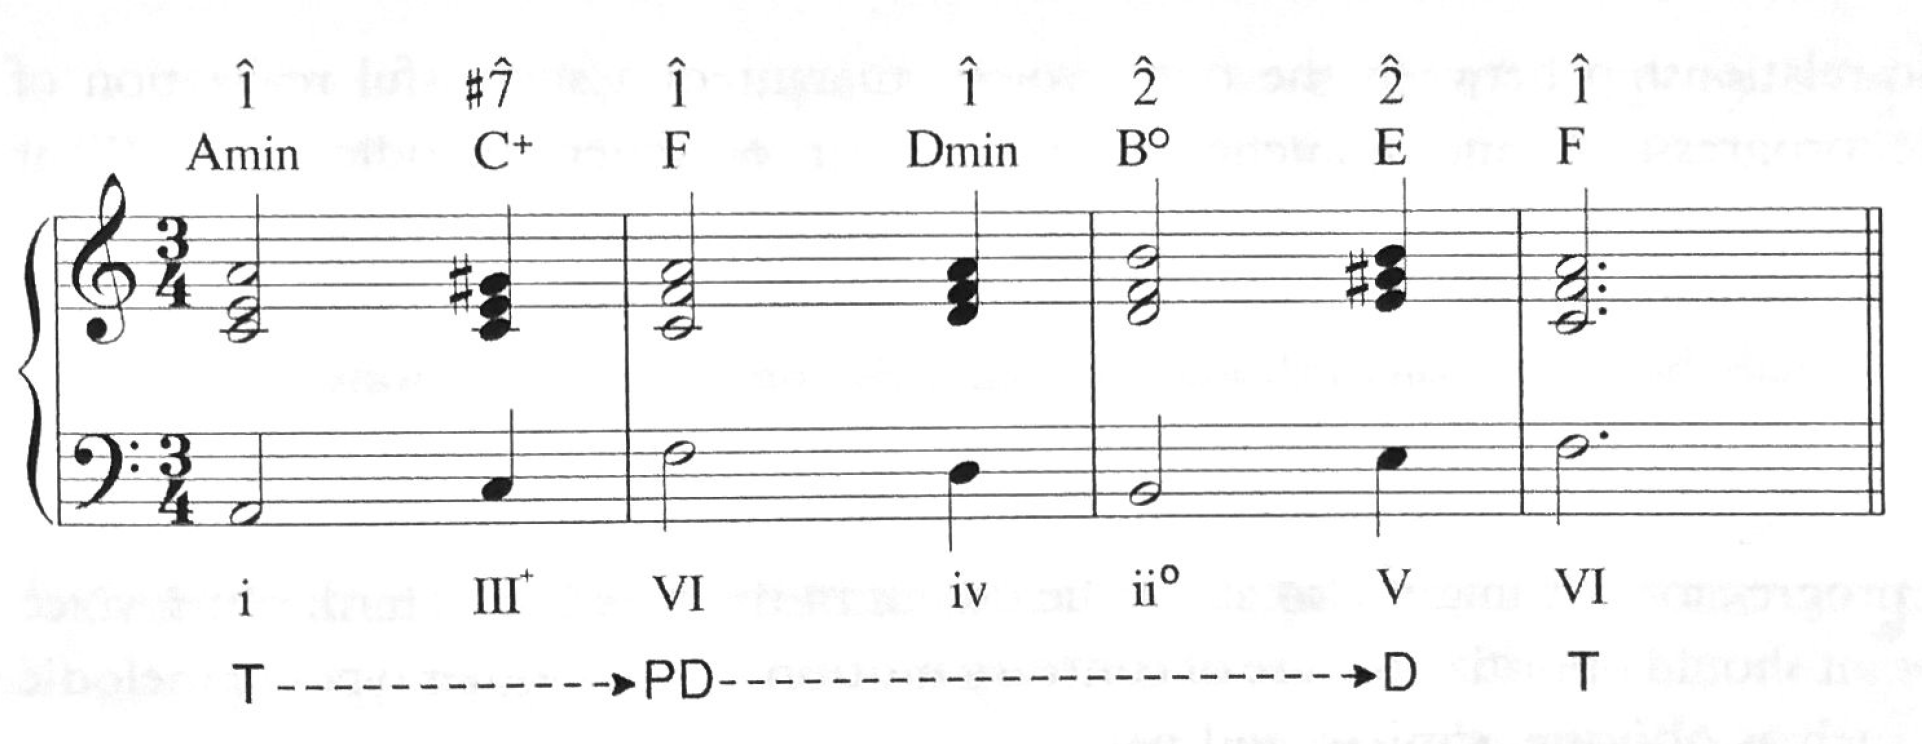
\includegraphics[width=5in]{Terefenko_ex.png}
	\label{Terefenko_ex}
\end{figure}

The segmentation procedure Terefenko employs is sensitive and emblematic of latent-formalist jazz analyses: begin by assigning a rooted, tertian-stack roman numeral label to each sonority, and consult a table of functional assignments to determine the category to which each roman numeral belongs.  When the category assignment is ambiguous, fall back on a the local context of the phrase, tracing a quick hermeneutic loop designed to produce whichever functional label best fits the analyst's expectation for normative behavior in the local context.  In Terefenko's words, ``The surrounding harmonic context in which chords occur determines the analytical interpretation of these chords."\footnote{Terefenko, p.\ 33.}  If that is true, then the assignment of particular chords to functional categories does not depend (or, more charitably, does not \emph{only} depend) on their pitch structures, despite the fact that the rest of Terefenko's material on harmonic function makes repeated reference to pitch-based tables of harmonic functional categories.  The implied segmentation procedure is not \emph{a priori} consistent, and it requires foreknowledge of which contextual forces will override the pitch-based category assignments found in elementary descriptions of tonic, predominant, and dominant.

This hermeneutic circle at the heart of functional parsing renders harmonic analysis flexible and fertile, but it also renders any truly latent formalist system incomplete or circular.  If there is no explicit account given for how functional assignment is to be done without recourse to the analyst's preconceptions, the formalist parsing runs the risk of confirming any preconceptions the analyst has.  As I claimed in Chapter 1's discussion of Lerdahl \& Jackendoff -- also latent formalists, much more explicitly -- the ``rules" of syntax cannot be proven on the basis of analyses of this kind, as contextual parsing will allow the analyst to shoe-horn a wide variety of musical surfaces into the analyst's pre-existing theory of harmonic syntax.  Terefenko is able to avoid an explicit account of functional category assignment precisely because the paradigm under which he operates assumes one implicitly: the pedagogical analysis of particular passages implies a set of top-down ``rules" to be taught to the student, and the application of those rules results in claims about the music at hand.  Whether those claims are meant to encompass how the teacher hears the music, how the student ought to hear the music, or something about the structure of the music independent of a hearer cannot readily be determined within the paradigm's framework.

%Wollheim's objection motivates my project
Latent functional analysis for pedagogical purposes may yet be re-writable under a temporal syntactic paradigm, but Wollheim's segmentation objection must first be dispatched: the data-driven temporal segmentation and clustering performed in chapters 2-4 is an attempt to do so.  Where Bois cannot separate elements within the Grebo mask, chapter 2 suggests that ``chords" or ``sonorities" might be extracted from YJaMP based on their temporal properties -- that we can consistently partition the notes of a performance based on the entropies of time-window note distributions and statistical patterns of inter-onset timing.  Where Bois cannot give an account of what general categories of syntactic behavior might exist for elements of the mask, and where Terefenko assumes pre-existing western-classical functions, chapter 3 suggests that statistics regarding temporal behavior on different time scales can serve as a ground for a kind of syntactic functionality.  And where Bois cannot provide meaningful rules assigning elements of the mask to syntactic categories or ordering them, and where Terefenko must rely on hermeneutic application of western-classical functional patterns, chapter 4 suggests that clustering chords based on similarities in their PCA-reduced temporal properties provides a starting point for functional assignment independent of analytical pre-conceptions.  Unlike in Wollheim's art-theoretical critique, a corpus of jazz piano harmony permits linguistically-inspired latent formalist description accountable to musical data.  Whether the resulting description still permits productive hermeneutic engagement with individual tunes for students and analysts is an open question.

\section{Affordances and limits of a new (or many) paradigm(s)}
%Is this, in fact, generalizable to a wider class of theory?  Bring in formalism, digital archives, the affordances of my corpus, and the necessity of both shoring up and quarantining formalism, leaving space for historical, contextual style analysis that can accomplish the remaining goals from the old paradigm.

%rehabilitate analysis from new paradigm: indicate that Terefenko uses two different paradigms, and that single-piece analysis under my paradigm also requires supplementation, either hermeneutically or with some other process.  But that my connection of rules to particulars is different.

%Chord-scale theory might interact well with temporal syntax?  Cue Levine jazz theory book

%Give specific, on-the-ground, new-paradigm claim examples!

%Bring it home.


